\section{Method}
\label{sec:method}

The decision making agents in this paper are tested on several randomly
generated transects.  They are repeatedly presented with an object to sample
and have to make the choice to either take a sample or continue travelling
along the transect.  Like the Robbins' secretary problem the agents are not
permitted to backtrack to avail of a previous opportunity.


Figure \ref{fig:transect} gives an example of a simulated transect. As we can
see there are sampling opportunities of different types scattered along the
path that the robot travels along.  

\begin{figure}[htpd!]
	\centering 
	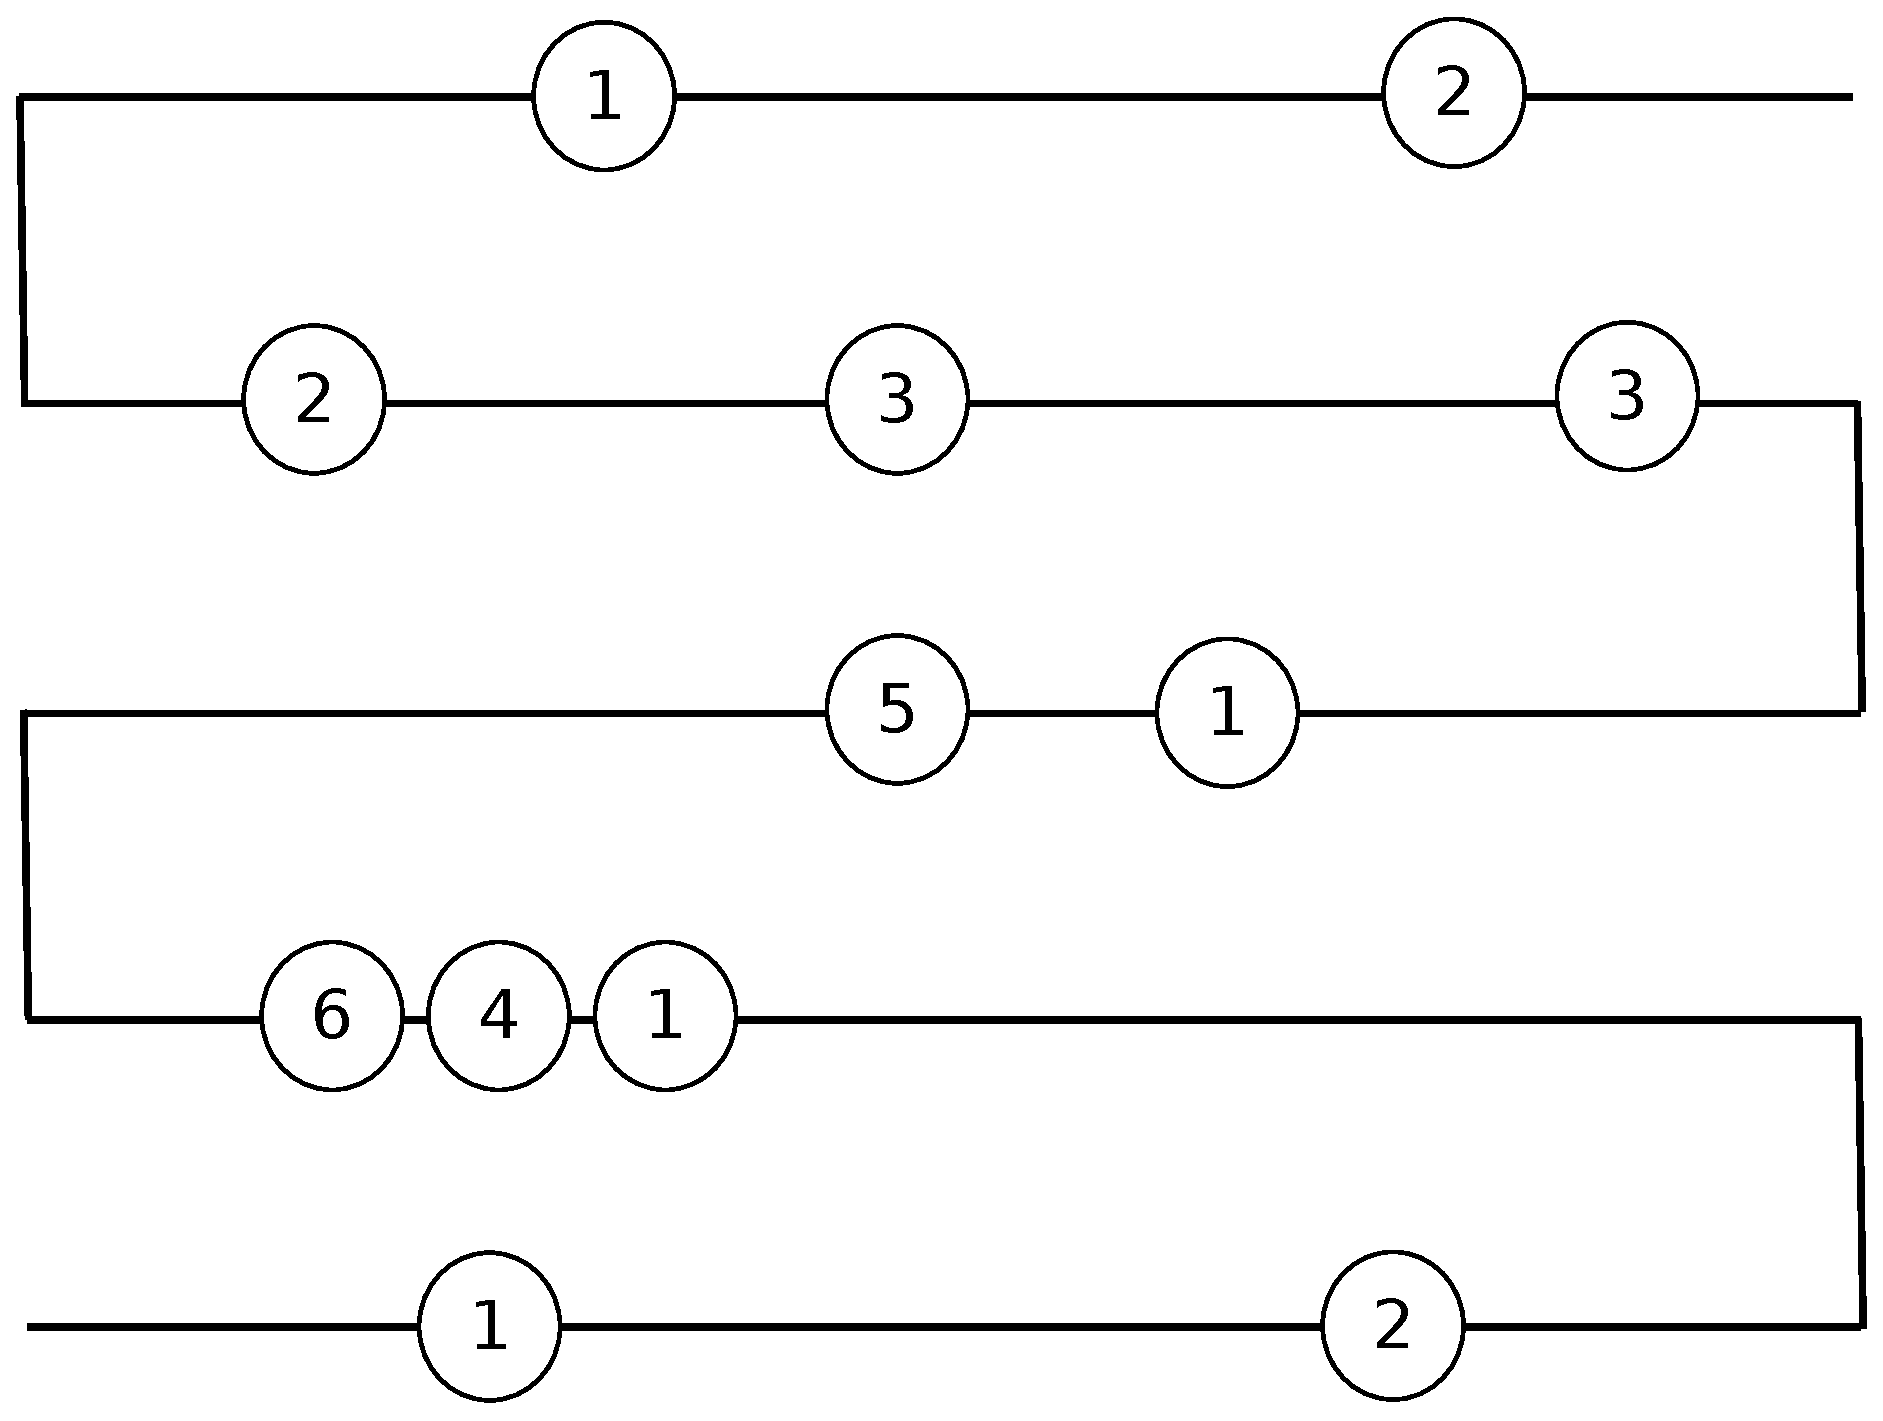
\includegraphics[width=0.8\textwidth]{transect}
	\caption{A cartoon illustrating a transect a robot might be encountering and how samping opportunities of different types may be distributed along it.  In the field the robot would start at one end of the path and follow it to the other end.  There is one path that the rover may follow across the terrain resulting in it encountering different types of sampling opportunities.}
	\label{fig:transect}
\end{figure}


The primary objective of the robot is to learn distributions behind different
classes of objects.  For example they may be the probability distribution
governing the density of sub surface microbial life in different classes of
soil.  Previous work have identified that texture information can successfully
classify different types of soil material \cite{trey_and_thompson_image_return_paper}.
We imagine that the classes of objects in
this research could correspond to those soil classes.



\subsection{Experiment}

The experiment presented in this paper is a modification of the experiments
presented in \cite{furlong2014sequential} and \cite{furlong2014budgeting}.  In the
prior work agents were equipped with limited sampling budgets.  In this
experiment the agents have an unlimited capacity to take samples, but the time
to take the sample is non-zero and there is an overall limit on the duration of
the mission.

As with the previous experiments the agents are not permitted to back track in
the hopes of getting a better opportunity.  The primary reason is to constantly
drive the robot to the end of its exploration mission.  Coverage is an
important part of exploration and permitting.  Additionally making decisions
between a current opportunity, a hypothetical future, and any number of
previously seen but unsampled opportunities is considered a more complex
problem and outside the scope of this paper.

In the experiment there are six different kinds of objects the agent may
encounter.  They each have their own arrival rate and their appearance along
the transect are generated with a poisson process.  In this paper the arrival
rates of the different sampling opportunities do not change over the course of
the experiment.  While this is almost certainly not the case for long range
traversals like those seen in the Life in the Atacama Desert Project it is a
reasonable approximation for shorter-range traverses.

\subsection{Algorithms}

	% This is only relevant in the larger work.
	% - figure method.3: texture cam, raw image and texture labelled image.

	The experiment builds on prior work.  Here we present three algorithms that are being testing on the simulated transect described above.

\subsubsection{Uniform Sampling}

The Uniform Sampling algorithm attempts to distribute the number of samples it
can collect evenly between the different types of objects present on the
transect.  This is chosen because it was a robustly successful algorithm, as
seen in the prior work \cite{furlong2014sequential} and \cite{furlong2014isairas}.

The Uniform Sampling algorithm does not consider the time remaining in the
transect, nor the time to complete sampling.

\subsubsection{Foraging}

The foraging algorithm is an attempt to maximize the productivity of the learning agent along the transect.  We attempt to maximize the number of bits learned per unit time.

The reward for sampling a class is an analog for the definition of surprise as
defined by the Koch et al {cite papers}.  Koch looked at the change in the
distribution that resulted in a Bayesian update.  Because this work uses a
non-parametric kernel density estimation we compare
$\log\left(\frac{\hat{p}(x|D\cup \left\{x\right\})}{\hat{p}(x|D)}\right)$.  To
be compatiable with optimal foraging algorithms, specifically the Marginal
Value Theorem of Charnov \cite{charnov1973optimal} the reward function must
have dimishing returns.  In the case of information update the Bayes Factor
will eventually converge to approximately 1, likewise our estimated empirical
bayes factor.  We take the log of this approximation such that it converges to
zero as more samples are collected.


	- figure method.2: The reward function as samples are given to it, for two or three different distributions.

	- Combining foraging models with bandit literature 
		- The previous work on foraging assumed an inherent value to
			options that the agent cared about.  Specifically, energy stored up.
		- We use a valuation model taken from bandit literature.  
		- We use the reward function from Koch's attention models
		- We use the decision making process from foraging. 
		- We add the concept of multi-arrival rate things, awareness of time limits.
	- Previous work had a limit on the number of samples it could take
		- We realized that the actual quantity that limits the exploration process
			is time.
		- By limiting the time and (in this case) relaxing the limit on sample sizes we more accurately deal with productivity.  
	- This experiment models a type of prospecting where the number of samples isn't limited but they do take time. 
	- To that end we are looking at productivity.

	-  This experiment is more akin to contextual bandits.  
	- The image represents a context, the NIRVSS 
	- Apply texturecam classification of a scene, as the context
	- the choice is to sample or continue

	- Productivity 


